\chapter{Resampling}

\section{Aliasing}

\begin{figure}[H]
  \centering
  \label{fig:aliasing_example}
  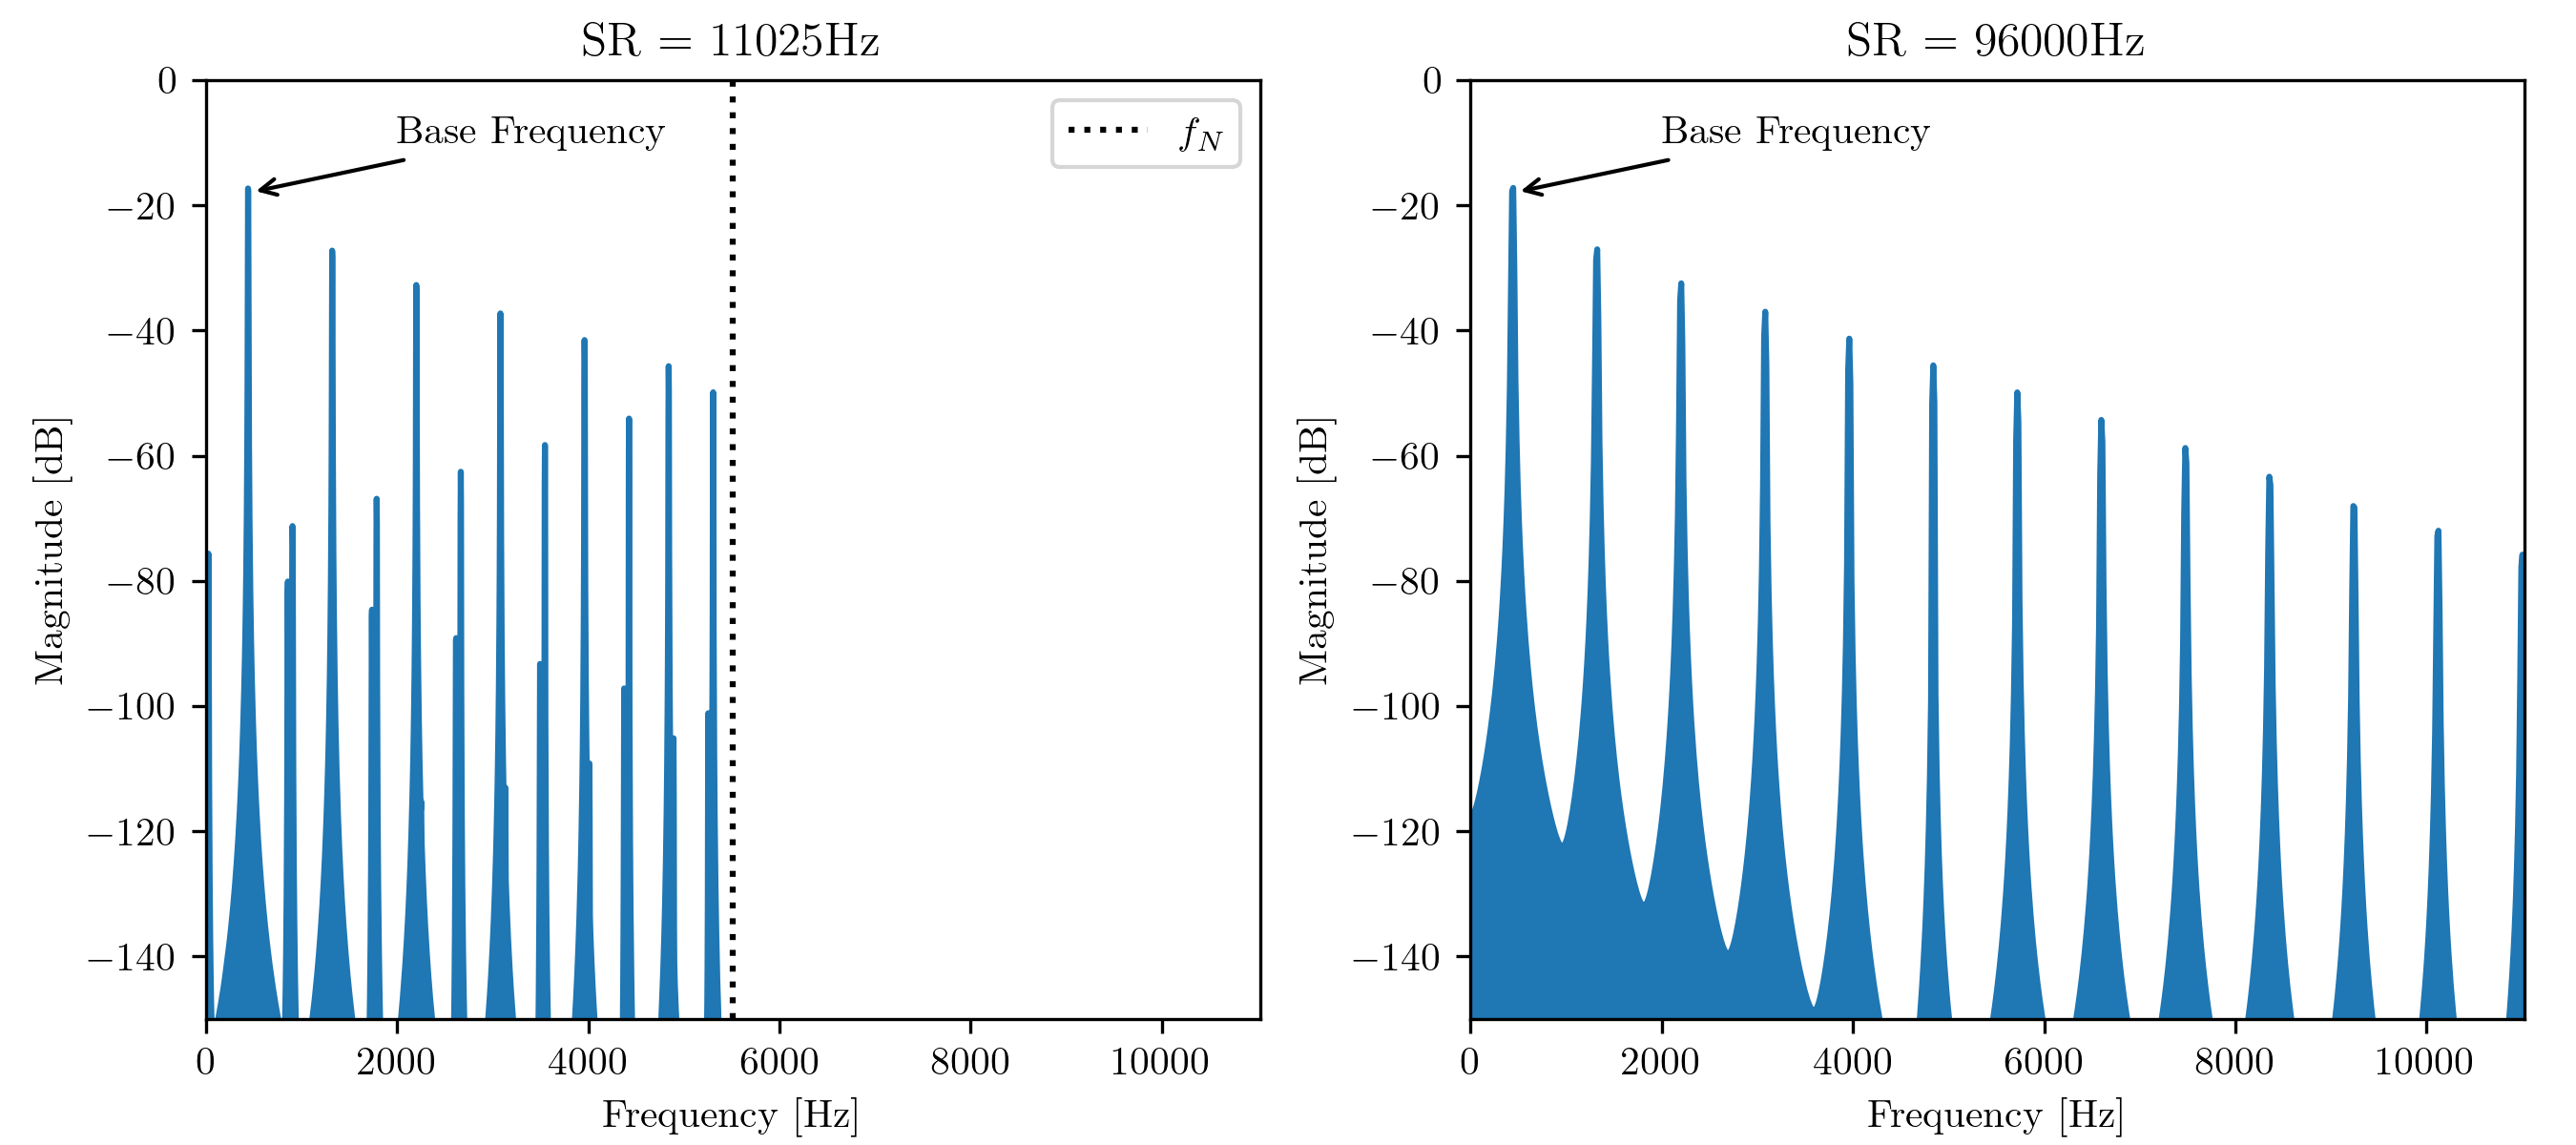
\includegraphics[width=\textwidth]{Pictures/aliasing_example.png}
  \caption{A \SI{440}{Hz} sine wave passed through $\omega(x) = \tanh(8x) \cdot\frac{1}{8}$ at two sample rates. The reflection
    around the Nyquist frequency can very clearly be seen at \SI{11025}{Hz}.}
\end{figure}

\begin{figure}[H]
  \centering
  \label{fig:resampled_tanh}
  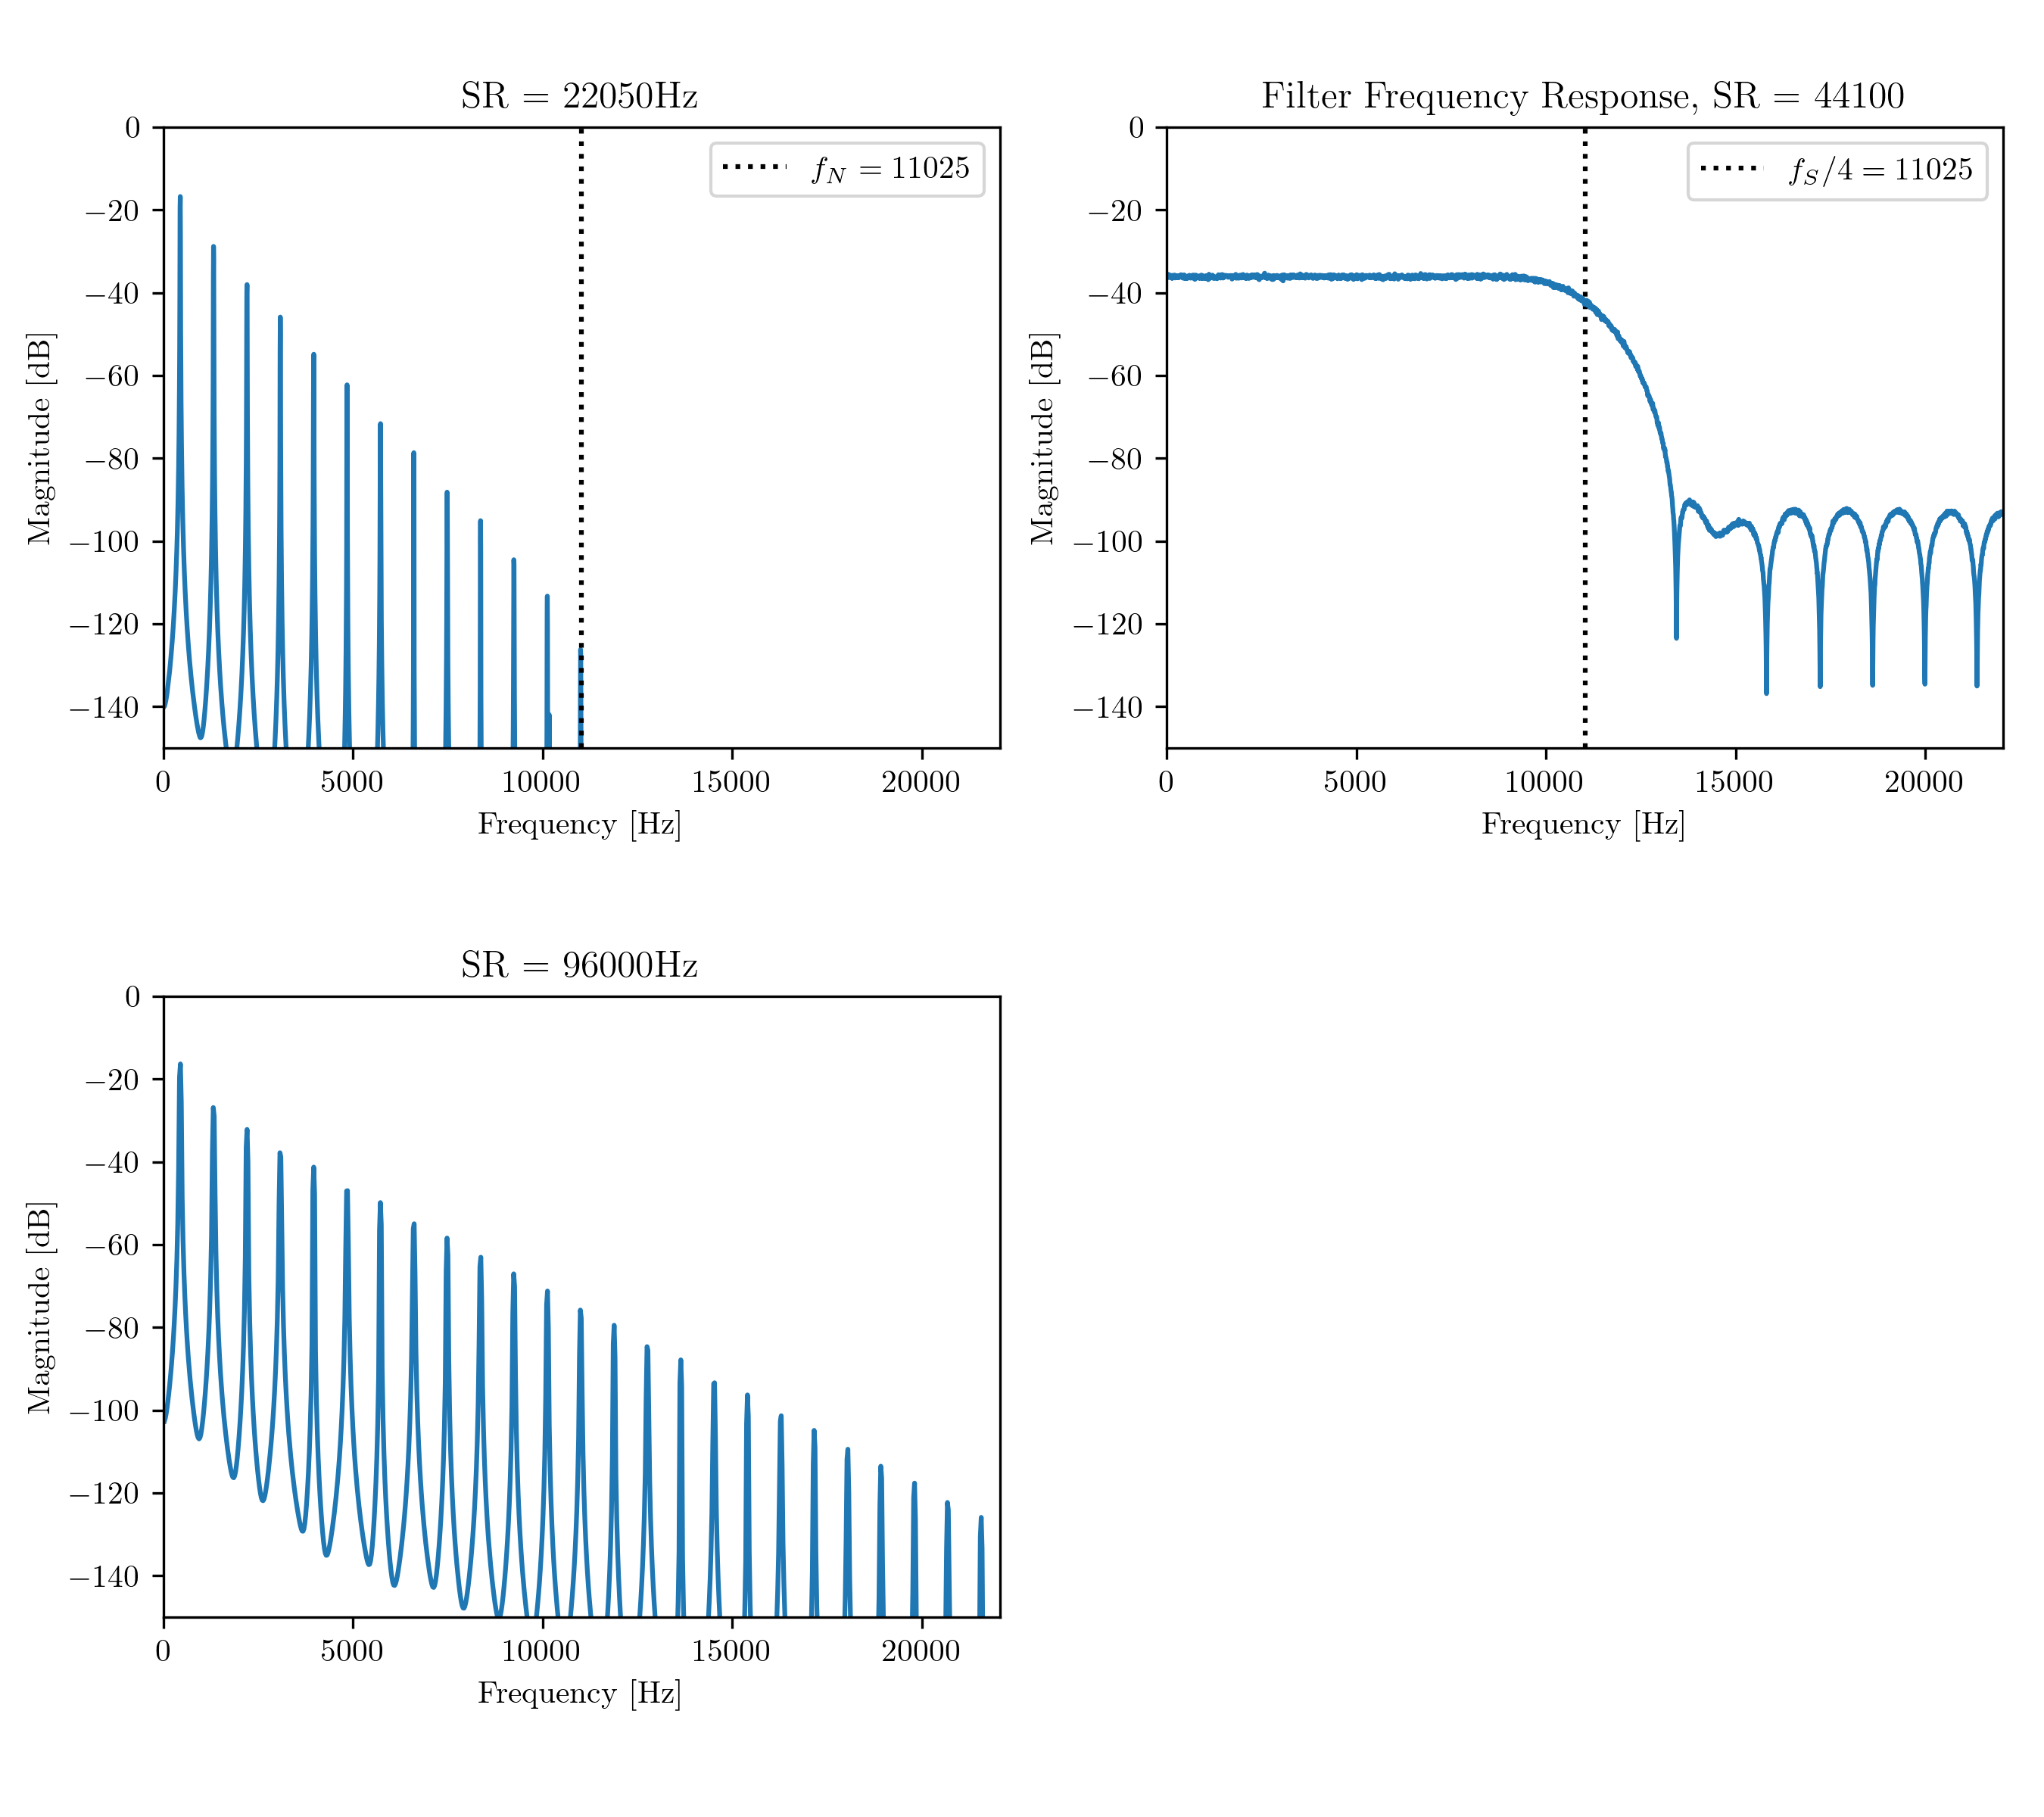
\includegraphics[width=\textwidth]{Pictures/resampled_tanh.png}
  \caption{The same nonlinear transform, but applied through1}
\end{figure}

\section{Oversampling for Alias reduction}
\section{Interpolation}
\section{Decimation}
\section{Resampling block}

\todo{argue this model of resampling instead of different in/out rates}

\begin{figure}[H]
  \centering
  \label{fig:block_resample}
  \includestandalone[]{Pictures/block_resample}
  \caption{The resample block as implemented in the EDA library}
\end{figure}

\subsection{C++ Implementation}
